\begin{frame}{GPRS et construction de backdoor}
    \large{\centerline{\textbf{Ne JAMAIS faire confiance à de la crypto propriétaire!}}}

\end{frame}

%------------------------------------------------
%------------------------------------------------

\begin{frame}{Make GEA great again \FiveStar\FiveStar\FiveStar \hfill 3 résolutions}
    \begin{columns}[c]
        \column{.45\textwidth}
        \begin{center}                  
            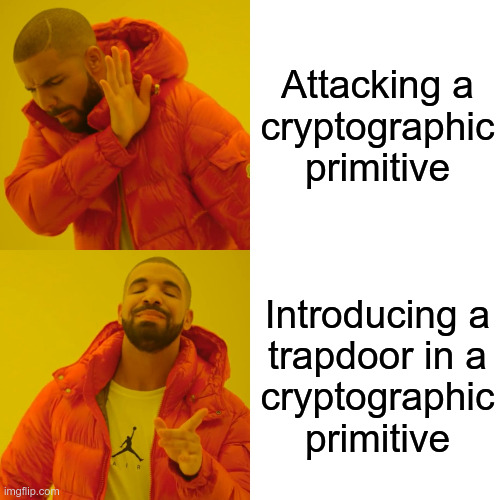
\includegraphics[width=0.9\textwidth]{img/meme/gea-intro.png}
        \end{center}

        \column{.65\textwidth} % 
           \begin{outline}
                \1 Objectifs : 
                    \2 Insérer une backdoor dans un stream-cipher LSFR
                \1 Données :
                    \2 Le code source
                    \2 Sagemath...
           \end{outline}
    \end{columns}
\end{frame}

%------------------------------------------------
%------------------------------------------------

\begin{frame}{Communication avec le serveur}
    \begin{columns}
        \column{0.5\textwidth}
        \begin{center}                  
            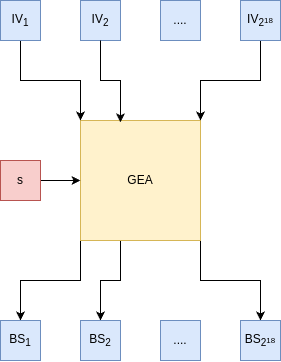
\includegraphics[width=0.7\textwidth]{img/crypto/gea/server.png}
        \end{center}
        \column{0.50\textwidth}
        \begin{itemize}
            \item $2^{18}$ IVs connus donnent $2^{18}$ BitStreams connus sur 64 bits
            \item Environ 10 minutes de génération
            \item Objectif : retrouver le secret $\u{s}$
        \end{itemize}
    \end{columns}

\end{frame}


\begin{frame}{GPRS et GEA}
    \begin{columns}
        \column{0.5\textwidth}
        \textbf{GPRS (General Packet Radio Service)}
        
        \vspace{0.3cm}

        \begin{center}
            \begin{tabular}{c c}
                \hline
                \textbf{Techno} & \textbf{Débit} \\
                \hline
                2G     & ~30 kbps \\
                GPRS    & ~ 100 kbps \\
                EDGE    & ~ 200 kbps \\
                3G      & ~ 1 Mbps \\
                \hline
            \end{tabular}
        \end{center}
        
        \vspace{0.3cm}
                
        \begin{outline}
            \1 Envoi de données par paquets
                \2[$\rightarrow$] Web, MMS, email amélioré
        \end{outline}

        \vspace{0.4cm}

        \pause 
        
        \column{0.55\textwidth}
        \textbf{GEA (GPRS Encryption Algorithm)}
        
        \vspace{0.5cm}
               
        \begin{itemize}
          \item Versions GEA1 à GEA5
          \item ETSI (European Telecommunications Standards Institute), 1998
        \end{itemize}           

        \begin{tcolorbox}
            "Doit se conformer aux restrictions européennes en vigueur sur les exports nationaux de la cryptographie"
        \end{tcolorbox}
        
        \begin{itemize}        
          \item GEA1 et GEA2 vulnérables 
        \end{itemize}
        
    \end{columns}
\end{frame}

\begin{frame}{GEA1}
    \only<1>{
        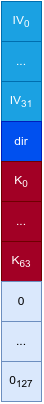
\includegraphics[width=\linewidth,height=0.8\textheight,keepaspectratio]{img/crypto/gea/mconverter/gea-1.png}
    }
    \only<2>{
        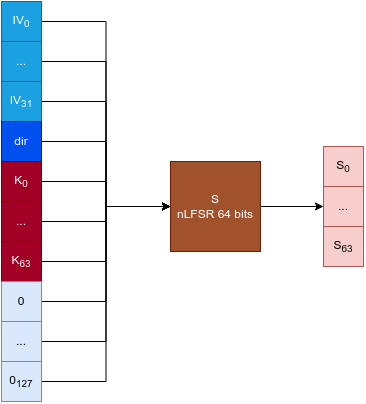
\includegraphics[width=\linewidth,height=0.8\textheight,keepaspectratio]{img/crypto/gea/mconverter/gea-2.png}
    }
    \only<3>{
        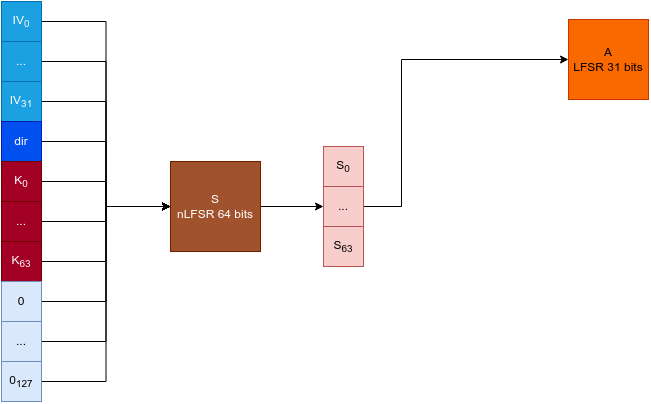
\includegraphics[width=\linewidth,height=0.8\textheight,keepaspectratio]{img/crypto/gea/mconverter/gea-3.png}
    }
    \only<4>{
        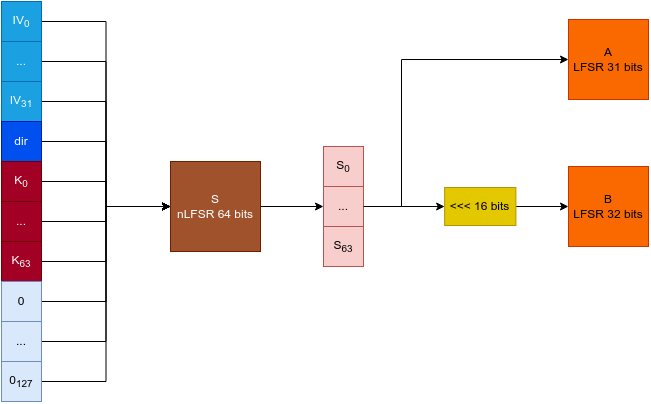
\includegraphics[width=\linewidth,height=0.8\textheight,keepaspectratio]{img/crypto/gea/mconverter/gea-4.png}
    }
    \only<5>{
        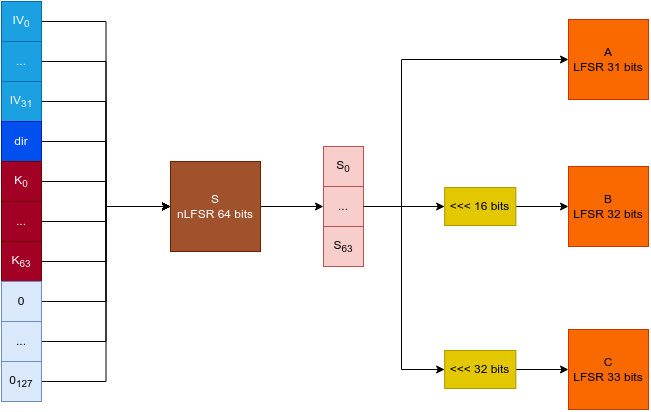
\includegraphics[width=\linewidth,height=0.8\textheight,keepaspectratio]{img/crypto/gea/mconverter/gea-5.png}
    }
    \only<6>{
        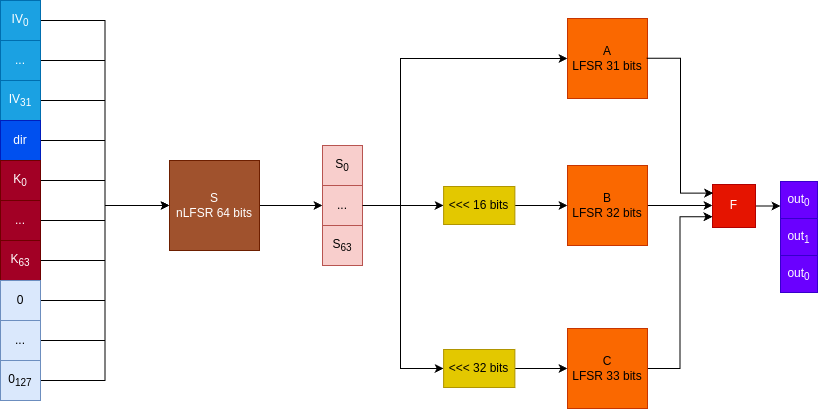
\includegraphics[width=\linewidth,height=0.8\textheight,keepaspectratio]{img/crypto/gea/mconverter/gea-6.png}
    }
\end{frame}

\begin{frame}{Sur les LFSRs de Galois (Linear Feedback Shift Register)}
    \begin{columns}[c]
        \column{.45\textwidth}
        
        \begin{center}                  
            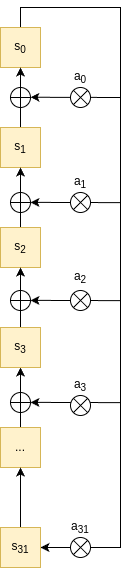
\includegraphics[width=0.23\textwidth]{img/crypto/gea/lfsr.png}
        \end{center}
        \pause
        \column{.55\textwidth} % 

\[\left\{
    \begin{array}{c c c c c}
        s_0 &\leftarrow & s_1 &\textcolor{orange}{+}& \textcolor{orange}{a_0s_0}\\
        s_1 &\leftarrow & s_2 &\textcolor{orange}{+}& \textcolor{orange}{a_1s_0}\\
        &\vdots& \\
        s_{30} &\leftarrow & s_{31} &\textcolor{orange}{+}& \textcolor{orange}{a_{30}s_0}\\
         s_{31} &\leftarrow & 0 &\textcolor{orange}{+}& \textcolor{orange}{a_{31}s_0}\\
    \end{array}
\right.\]

\[\left(\begin{array}{c}
        s_0 \\
        s_1 \\
        \vdots \\
        s_{30}\\
        s_{31}\\
    \end{array}\right)
    \leftarrow
    \left(
    \begin{array}{c c c c c }
        \textcolor{orange}{a_0} & 1 & 0 & \dots & 0\\
        \textcolor{orange}{a_1} & 0 & 1 & &0\\
        \vdots& \vdots & & \ddots &  \\
        \textcolor{orange}{a_{30}} & 0 & \dots &0 & 1\\
        \textcolor{orange}{a_{31}} & 0 & \dots &0 & 0\\
    \end{array}
\right)\left(\begin{array}{c}
        s_0 \\
        s_1 \\
        \vdots \\
        s_{30} \\
        s_{31}\\
    \end{array}\right)\]
    \end{columns}

    \pause 
    
    \begin{outline}
        \1 Fait intervenir la matrice compagnon $G_P$ de $P = X^{32} + a_{31}X^{31} \dots +a_1 X +a_0$
    \end{outline}
\end{frame}

\begin{frame}{Dans le cadre de GEA1}

\begin{center}                  
    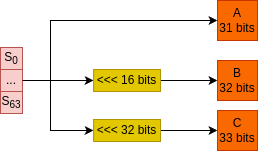
\includegraphics[width=0.35\textwidth]{img/crypto/gea/zoom.png}
\end{center}

\begin{itemize}
    \item L'état initial de A, B, C est linéaire en l'entrée secrète $\u{\mathbf{s}}$
    
    \item On a les états $\k{\mathbf{M_A}}.\u{\mathbf{s}}$, $\k{\mathbf{M_B}}.\u{\mathbf{s}}$, $\k{\mathbf{M_C}}.\u{\mathbf{s}}$ des matrices de taille $31*64$, $32*64$, $33*64$
    \pause

    \item $T_{AC} := \ker(\k{\mathbf{M_A}}) \bigcap \ker(\k{\mathbf{M_C}})$ est de dimension 24 et $T_{AC}\bigcap \ker(\k{\mathbf{M_B}}) = \{0\}$

    \item Ceci donne une récupération en $2^{37}$ appels d'oracle, $2^{40}$ bruteforces, en utilisant $2^8$ tables de $2^{24}*89$ bits (48 Go)\footnote{\cite{cryptoeprint:2021/819}}
\end{itemize}
\end{frame}

%\begin{frame}{intuition de l'attaque}
%pas une priorité
%\end{frame}

\begin{frame}{Et dans le cas du challenge?}
B est rotate de 21 (et non 16) et C est rotate de 42 (et non 32) 
\begin{outline}
    \1 Quels polynômes donnent une attaque?
    \pause
    \1 Comment les polynômes de GEA1 ont été trouvés? \footnote{\cite{cryptoeprint:2021/829}}

        \pause 
        
    \begin{block}{Condition d'appartenance au kernel après rotation}
    Si $\mathbf{t}=(t_0,\dots,t_{63})\in\ker(\mathbf{M_A})$ où A est un LFSR de polynôme de Galois primitif $P_A$ dont l'entrée est rotation de $k$, alors

    \[P_A \;|\; \left(t_0X^{k}+\dots +t_{k-1}X^1\right) + \left(t_{k}X^{64} + \dots + t_{63}X^{k+1}\right) =\displaystyle\sum_{i=0}^{k-1} t_i X^{k-i} + \displaystyle\sum_{i=k}^{63} t_i X^{64-i+k}\]

    Par exemple, en l'absence de rotation, $P_A \;|\; \displaystyle\sum_{i=0}^{63} t_i X^{64-i}$
    \end{block}
\end{outline}
\end{frame}

\begin{frame}{Partage de kernel}
On va plutôt partir du kernel et chercher des polynômes qui ont ce kernel en commun \footnote{\cite{cryptoeprint:2021/829}}
\begin{block}{Condition d'appartenance au kernel après rotation}
    Soit deux LSFR A et B. A n'est pas shifté et B est shifté de k. Si $\mathbf{t}=(t_0,\dots,t_{63})\in\ker(\mathbf{M_A})\bigcap \ker(\mathbf{M_B}) := T_{A,B}$ alors

\[P_A \;|\; \displaystyle\sum_{i=0}^{63} t_i X^{64-i} \text{  et  } P_B \;|\; \displaystyle\sum_{i=0}^{k-1} t_i X^{k-i} + \displaystyle\sum_{i=k}^{63} t_i X^{64-i+k}\]

    De plus, $\dim(T_{A,B}) \geq r$ où $X^r$ divise les deux polynômes de droite
    
    \pause
    
    \small{car alors $\mathbf{t_i}=(0,...,0,t_0,\dots,t_{63-i})\in T_{A,B}$ pour $i<r$}
    \end{block}
\end{frame}

\begin{frame}{Un exemple jouet}
\begin{outline}
    \1  Si B est shifté de 32 et que l'on cherche $T_{A,B}$ de dimension 31, on cherche $\mathbf{t}$ tel que

\[X^{31} \;|\; \displaystyle\sum_{i=0}^{63} t_i X^{64-i} \text{  et  } X^{31} \;|\; \displaystyle\sum_{i=0}^{32-1} t_i X^{32-i} + \displaystyle\sum_{i=32}^{63} t_i X^{64-i+32}\]

\pause

\1 L'équation gauche force $t_{63}\mapsto t_{34}$ à zéro. L'équation droite force $t_{1}\mapsto t_{31}$ à zéro.
    \2 Bruteforce exhaustif de $t_0,t_{32}$ et $t_{33}$ ($8$ solutions)

\pause 

\1 On cherche alors 
    \2 $P_A\;|\;t_0X^{64} + t_{32}X^{32} + t_{33}X^{31}$ 
    \2 $P_B\;|\; t_{32}X^{64} + t_{33}X^{63} + t_0X^{32} $

\pause

\1 Tous polynômes \textbf{primitifs de la bonne taille}  produiront le bon kernel
\end{outline}

$\Rightarrow$ La dimension du kernel est bornée par le shift \textbf{relatif}
\end{frame}

\begin{frame}{Exploiter les shifts}
\begin{itemize}
    \item GEA1 : Shifts 16 et 32 $\Rightarrow$ kernel joint maximal de dimension 32 entre A et C 
    \pause
    \item CTF : Shifts 21 et 42 $\Rightarrow$ kernel joint maximal de dimension 22 entre C et A
    \pause
    \item Exploiter la symétrie, existe-t-il un $T_{A,B,C}$ grand?
\end{itemize}

\pause

\begin{center}
OUI! On trouve par bruteforce un $T_{A,B,C}$ de dimension 16
\end{center}

\pause

\begin{small}
\begin{itemize}
    \item $f = X^{31} + X^{27} + X^{26} + X^{25} + X^{23} + X^{17} + X^{15} + X^{13} + X^{11} + X^9 + X^7 + X^6 + X^5 + X^3 + X^2 + X + 1$
    \item $g = X^{32} + X^{30} + X^{27} + X^{23} + X^{18} + X^{17} + X^{16} + X^{12} + X^{11} + X^9 + X^8 + X^6 + X^4 + X^3 + X^2 + X + 1$
    \item $h = X^{33} + X^{29} + X^{28} + X^{27} + X^{25} + X^{24} + X^{23} + X^{22} + X^{20} + X^{19} + X^{18} + X^{17} + X^9 + X^6 + X^5 + X^4 + X^3 + X + 1$
\end{itemize}
\end{small}

\pause
\[\mathbb{F}_2^{64} = T_{A,B,C}\oplus  V \text{ et donc } \u{\mathbf{s}} = \u{\mathbf{s}_{T}}+\u{\mathbf{s}_V}\]

Aussi, $\u{\mathbf{s}}\mapsto (\k{\mathbf{M_A}}.\u{\mathbf{s}},\k{\mathbf{M_B}}.\u{\mathbf{s}},\k{\mathbf{M_C}}.\u{\mathbf{s}}) =(\k{\mathbf{M_A}}.\u{\mathbf{s}_V},\k{\mathbf{M_B}}.\u{\mathbf{s}_V},\k{\mathbf{M_C}}.\u{\mathbf{s}_V})$ n'a que 48 bits d'entropie
    
\end{frame}

\begin{frame}{Attaque finale}

\begin{outline}
    \1 Objectif : Grace aux $2^{18}$ bitstreams , trouver l'un des $\u{\mathbf{s}}$, pour revenir à la clef
    
    \pause
    
    \1 $\mathbb{F}_2^{64} = T_{A,B,C}\oplus V = T_{A,B,C} \oplus  X \oplus  Y \text{ et donc } \u{\mathbf{s}} = \u{\mathbf{s}_{T}}+\u{\mathbf{s}_{X}}+\u{\mathbf{s}_Y}$
    \2 $X$ de dimension 30 et $Y$ de dimension 18
    \pause
    \2 Bitstream $BS(\u{\mathbf{s}}) = BS(\u{\mathbf{s}_{X}}+\u{\mathbf{s}_Y})$
\pause
\1 Précalcul des $2^{30}$ valeurs de $BS(\mathbf{s}_{X}+0)$ dans une hashmap $H$
\pause
    \2 $H : BS \text{(64 bits)} \mapsto \mathbf{s}_{X} \text{(30 bits)}$
    \pause
    \2 Un bitstream fait $64$ bits $\Rightarrow$ $64*2^{30}=8Go$ de stockage
    \pause
\1 Statistiquement, l'un des $\u{\mathbf{s}_Y}=0$
\pause
    \2 Le $BS(\u{\mathbf{s}})$ associé est dans $H$
    \pause
    \2 $H$ nous donne $\u{\mathbf{s}_{X}}$ 
    \pause
\1 On retrouve $\u{\mathbf{s}} = \u{\mathbf{s}_{T}}+\u{\mathbf{s}_{X}}+0$ ($2^{16}$ valeurs de $\u{\mathbf{s}_{T}}$)
\1 Avec $\u{\mathbf{s}}$ et $\k{\mathbf{IV}}$ associé, on retrouve la clef

\1 Total : $2^{30} + 2^{16}$ opérations, 8Go de mémoire  \hfill \flag
\end{outline}

\end{frame}

